


% Gradient Info
  
\tikzset {_rsx50m4nz/.code = {\pgfsetadditionalshadetransform{ \pgftransformshift{\pgfpoint{89.1 bp } { -128.7 bp }  }  \pgftransformscale{1.32 }  }}}
\pgfdeclareradialshading{_kzqb0ap3i}{\pgfpoint{-72bp}{104bp}}{rgb(0bp)=(1,1,1);
rgb(0bp)=(1,1,1);
rgb(25bp)=(0.48,0.15,0.15);
rgb(400bp)=(0.48,0.15,0.15)}

% Gradient Info
  
\tikzset {_4g38zib54/.code = {\pgfsetadditionalshadetransform{ \pgftransformshift{\pgfpoint{0 bp } { 0 bp }  }  \pgftransformrotate{0 }  \pgftransformscale{2 }  }}}
\pgfdeclarehorizontalshading{_pflu9vvmw}{150bp}{rgb(0bp)=(0,0.2,0.2);
rgb(37.5bp)=(0,0.2,0.2);
rgb(50bp)=(0.02,0.76,1);
rgb(62.5bp)=(0,0.2,0.2);
rgb(100bp)=(0,0.2,0.2)}
\tikzset{every picture/.style={line width=0.75pt}} %set default line width to 0.75pt        

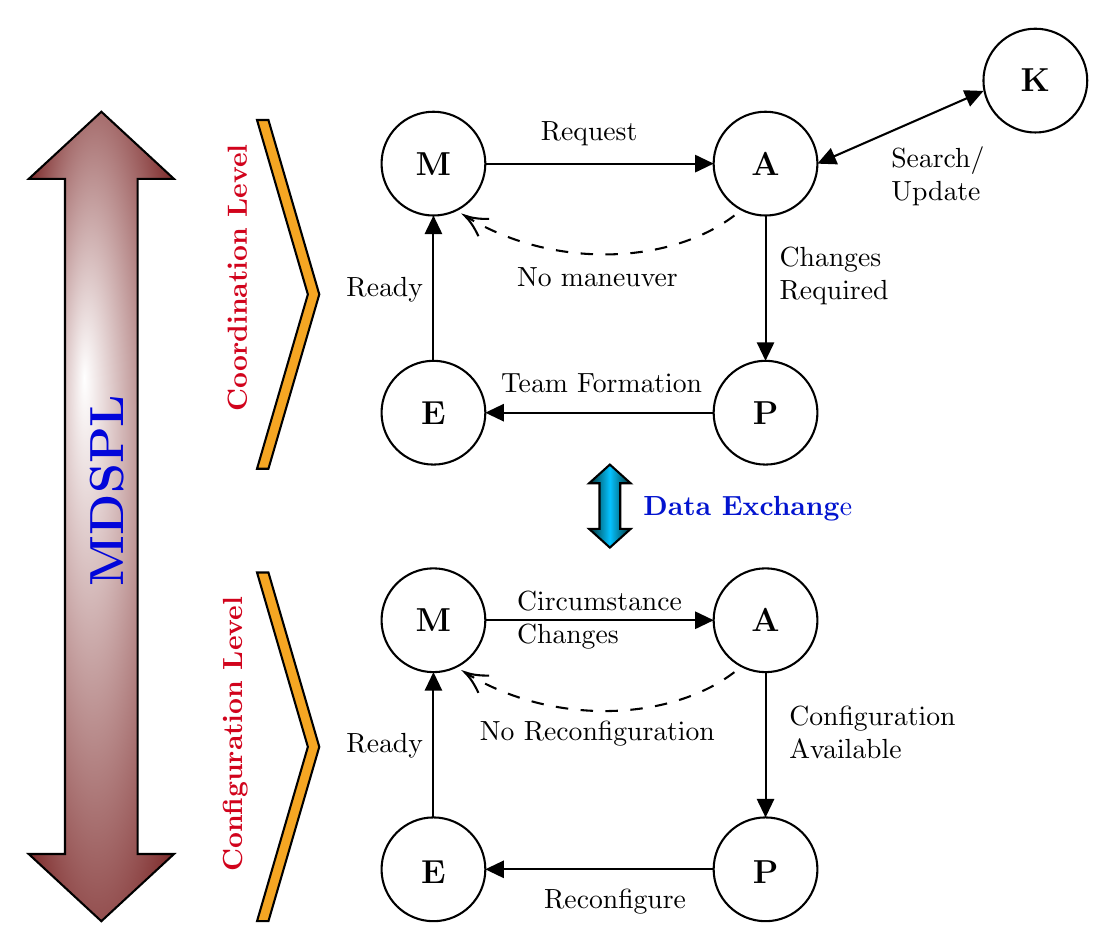
\begin{tikzpicture}[x=0.75pt,y=0.75pt,yscale=-1,xscale=1]
%uncomment if require: \path (0,473); %set diagram left start at 0, and has height of 473

%Up Down Arrow [id:dp782850436661098] 
\path  [shading=_kzqb0ap3i,_rsx50m4nz] (20,82.38) -- (55,50) -- (90,82.38) -- (72.5,82.38) -- (72.5,407.62) -- (90,407.62) -- (55,440) -- (20,407.62) -- (37.5,407.62) -- (37.5,82.38) -- cycle ; % for fading 
 \draw   (20,82.38) -- (55,50) -- (90,82.38) -- (72.5,82.38) -- (72.5,407.62) -- (90,407.62) -- (55,440) -- (20,407.62) -- (37.5,407.62) -- (37.5,82.38) -- cycle ; % for border 

%Shape: Circle [id:dp8183502258316318] 
\draw   (190,75) .. controls (190,61.19) and (201.19,50) .. (215,50) .. controls (228.81,50) and (240,61.19) .. (240,75) .. controls (240,88.81) and (228.81,100) .. (215,100) .. controls (201.19,100) and (190,88.81) .. (190,75) -- cycle ;
%Shape: Circle [id:dp6317302847731573] 
\draw   (350,75) .. controls (350,61.19) and (361.19,50) .. (375,50) .. controls (388.81,50) and (400,61.19) .. (400,75) .. controls (400,88.81) and (388.81,100) .. (375,100) .. controls (361.19,100) and (350,88.81) .. (350,75) -- cycle ;
%Shape: Circle [id:dp5409698763729759] 
\draw   (190,195) .. controls (190,181.19) and (201.19,170) .. (215,170) .. controls (228.81,170) and (240,181.19) .. (240,195) .. controls (240,208.81) and (228.81,220) .. (215,220) .. controls (201.19,220) and (190,208.81) .. (190,195) -- cycle ;
%Shape: Circle [id:dp7510782908406544] 
\draw   (350,195) .. controls (350,181.19) and (361.19,170) .. (375,170) .. controls (388.81,170) and (400,181.19) .. (400,195) .. controls (400,208.81) and (388.81,220) .. (375,220) .. controls (361.19,220) and (350,208.81) .. (350,195) -- cycle ;
%Straight Lines [id:da5662694326503737] 
\draw    (240,75) -- (347,75) ;
\draw [shift={(350,75)}, rotate = 180] [fill={rgb, 255:red, 0; green, 0; blue, 0 }  ][line width=0.08]  [draw opacity=0] (8.93,-4.29) -- (0,0) -- (8.93,4.29) -- cycle    ;

%Straight Lines [id:da5870438424369948] 
\draw    (375,100) -- (375,167) ;
\draw [shift={(375,170)}, rotate = 270] [fill={rgb, 255:red, 0; green, 0; blue, 0 }  ][line width=0.08]  [draw opacity=0] (8.93,-4.29) -- (0,0) -- (8.93,4.29) -- cycle    ;

%Straight Lines [id:da5401498459364277] 
\draw    (350,195) -- (243,195) ;
\draw [shift={(240,195)}, rotate = 360] [fill={rgb, 255:red, 0; green, 0; blue, 0 }  ][line width=0.08]  [draw opacity=0] (8.93,-4.29) -- (0,0) -- (8.93,4.29) -- cycle    ;

%Straight Lines [id:da838639879392216] 
\draw    (215,170) -- (215,103) ;
\draw [shift={(215,100)}, rotate = 450] [fill={rgb, 255:red, 0; green, 0; blue, 0 }  ][line width=0.08]  [draw opacity=0] (8.93,-4.29) -- (0,0) -- (8.93,4.29) -- cycle    ;

%Shape: Circle [id:dp5111748591406433] 
\draw   (480,35) .. controls (480,21.19) and (491.19,10) .. (505,10) .. controls (518.81,10) and (530,21.19) .. (530,35) .. controls (530,48.81) and (518.81,60) .. (505,60) .. controls (491.19,60) and (480,48.81) .. (480,35) -- cycle ;
%Straight Lines [id:da6073198118735847] 
\draw    (402.75,73.8) -- (477.25,41.2) ;
\draw [shift={(480,40)}, rotate = 516.37] [fill={rgb, 255:red, 0; green, 0; blue, 0 }  ][line width=0.08]  [draw opacity=0] (8.93,-4.29) -- (0,0) -- (8.93,4.29) -- cycle    ;
\draw [shift={(400,75)}, rotate = 336.37] [fill={rgb, 255:red, 0; green, 0; blue, 0 }  ][line width=0.08]  [draw opacity=0] (8.93,-4.29) -- (0,0) -- (8.93,4.29) -- cycle    ;
%Shape: Circle [id:dp7346161724442969] 
\draw   (190,295) .. controls (190,281.19) and (201.19,270) .. (215,270) .. controls (228.81,270) and (240,281.19) .. (240,295) .. controls (240,308.81) and (228.81,320) .. (215,320) .. controls (201.19,320) and (190,308.81) .. (190,295) -- cycle ;
%Shape: Circle [id:dp9313506421767208] 
\draw   (350,295) .. controls (350,281.19) and (361.19,270) .. (375,270) .. controls (388.81,270) and (400,281.19) .. (400,295) .. controls (400,308.81) and (388.81,320) .. (375,320) .. controls (361.19,320) and (350,308.81) .. (350,295) -- cycle ;
%Shape: Circle [id:dp15172584011360524] 
\draw   (190,415) .. controls (190,401.19) and (201.19,390) .. (215,390) .. controls (228.81,390) and (240,401.19) .. (240,415) .. controls (240,428.81) and (228.81,440) .. (215,440) .. controls (201.19,440) and (190,428.81) .. (190,415) -- cycle ;
%Shape: Circle [id:dp5193390537739596] 
\draw   (350,415) .. controls (350,401.19) and (361.19,390) .. (375,390) .. controls (388.81,390) and (400,401.19) .. (400,415) .. controls (400,428.81) and (388.81,440) .. (375,440) .. controls (361.19,440) and (350,428.81) .. (350,415) -- cycle ;
%Straight Lines [id:da7790158602823466] 
\draw    (240,295) -- (347,295) ;
\draw [shift={(350,295)}, rotate = 180] [fill={rgb, 255:red, 0; green, 0; blue, 0 }  ][line width=0.08]  [draw opacity=0] (8.93,-4.29) -- (0,0) -- (8.93,4.29) -- cycle    ;

%Straight Lines [id:da00012936718183331752] 
\draw    (375,320) -- (375,387) ;
\draw [shift={(375,390)}, rotate = 270] [fill={rgb, 255:red, 0; green, 0; blue, 0 }  ][line width=0.08]  [draw opacity=0] (8.93,-4.29) -- (0,0) -- (8.93,4.29) -- cycle    ;

%Straight Lines [id:da5416108782633927] 
\draw    (350,415) -- (243,415) ;
\draw [shift={(240,415)}, rotate = 360] [fill={rgb, 255:red, 0; green, 0; blue, 0 }  ][line width=0.08]  [draw opacity=0] (8.93,-4.29) -- (0,0) -- (8.93,4.29) -- cycle    ;

%Straight Lines [id:da20830974811893643] 
\draw    (215,390) -- (215,323) ;
\draw [shift={(215,320)}, rotate = 450] [fill={rgb, 255:red, 0; green, 0; blue, 0 }  ][line width=0.08]  [draw opacity=0] (8.93,-4.29) -- (0,0) -- (8.93,4.29) -- cycle    ;

%Up Down Arrow [id:dp4468819868142203] 
\path  [shading=_pflu9vvmw,_4g38zib54] (290,229) -- (300,220) -- (310,229) -- (305,229) -- (305,251) -- (310,251) -- (300,260) -- (290,251) -- (295,251) -- (295,229) -- cycle ; % for fading 
 \draw   (290,229) -- (300,220) -- (310,229) -- (305,229) -- (305,251) -- (310,251) -- (300,260) -- (290,251) -- (295,251) -- (295,229) -- cycle ; % for border 

%Chevron Arrow [id:dp7018991082889573] 
\draw  [fill={rgb, 255:red, 245; green, 166; blue, 35 }  ,fill opacity=1 ] (130,54) -- (135.5,54) -- (160,138) -- (135.5,222) -- (130,222) -- (154.5,138) -- cycle ;
%Chevron Arrow [id:dp5132381851000084] 
\draw  [fill={rgb, 255:red, 245; green, 166; blue, 35 }  ,fill opacity=1 ] (130,272) -- (135.5,272) -- (160,356) -- (135.5,440) -- (130,440) -- (154.5,356) -- cycle ;
%Curve Lines [id:da6114980910459762] 
\draw  [dash pattern={on 4.5pt off 4.5pt}]  (360,100) .. controls (328.82,123.76) and (272.64,125.96) .. (231.25,100.77) ;
\draw [shift={(230,100)}, rotate = 392.07] [color={rgb, 255:red, 0; green, 0; blue, 0 }  ][line width=0.75]    (10.93,-4.9) .. controls (6.95,-2.3) and (3.31,-0.67) .. (0,0) .. controls (3.31,0.67) and (6.95,2.3) .. (10.93,4.9)   ;

%Curve Lines [id:da827843564081892] 
\draw  [dash pattern={on 4.5pt off 4.5pt}]  (360,320) .. controls (328.82,343.76) and (272.64,345.96) .. (231.25,320.77) ;
\draw [shift={(230,320)}, rotate = 392.07] [color={rgb, 255:red, 0; green, 0; blue, 0 }  ][line width=0.75]    (10.93,-4.9) .. controls (6.95,-2.3) and (3.31,-0.67) .. (0,0) .. controls (3.31,0.67) and (6.95,2.3) .. (10.93,4.9)   ;


% Text Node
\draw (58,232.5) node  [color={rgb, 255:red, 2; green, 6; blue, 218 }  ,opacity=1 ,rotate=-270] [align=left] {\textbf{{\LARGE MDSPL}}};
% Text Node
\draw (120.5,130) node  [rotate=-270] [align=left] {\textbf{\textcolor[rgb]{0.82,0.01,0.11}{Coordination Level}}};
% Text Node
\draw (119.5,350) node  [rotate=-270] [align=left] {\textbf{\textcolor[rgb]{0.82,0.01,0.11}{Configuration Level}}};
% Text Node
\draw (215,75) node  [font=\large] [align=left] {\textbf{M}};
% Text Node
\draw (215,295) node  [font=\large] [align=left] {\textbf{M}};
% Text Node
\draw (375,75) node  [font=\large] [align=left] {\textbf{A}};
% Text Node
\draw (375,195) node  [font=\large] [align=left] {\textbf{P}};
% Text Node
\draw (215,195) node  [font=\large] [align=left] {\textbf{E}};
% Text Node
\draw (505,35) node  [font=\large] [align=left] {\textbf{K}};
% Text Node
\draw (375,416.5) node  [font=\large] [align=left] {\textbf{P}};
% Text Node
\draw (215,416.5) node  [font=\large] [align=left] {\textbf{E}};
% Text Node
\draw (375,295) node  [font=\large] [align=left] {\textbf{A}};
% Text Node
\draw (458,81) node   [align=left] {Search/\\Update};
% Text Node
\draw (290,60.5) node   [align=left] {Request};
% Text Node
\draw (408,129) node   [align=left] {Changes\\Required};
% Text Node
\draw (296,180.5) node   [align=left] {Team Formation};
% Text Node
\draw (191.5,135.5) node   [align=left] {Ready};
% Text Node
\draw (294,129.5) node   [align=left] {No maneuver};
% Text Node
\draw (294,349.5) node   [align=left] {No Reconfiguration};
% Text Node
\draw (295,295) node   [align=left] {Circumstance\\Changes};
% Text Node
\draw (426.5,349) node   [align=left] {Configuration\\Available};
% Text Node
\draw (302.5,430.5) node   [align=left] {Reconfigure};
% Text Node
\draw (191.5,355.5) node   [align=left] {Ready};
% Text Node
\draw (366.5,241) node  [color={rgb, 255:red, 74; green, 144; blue, 226 }  ,opacity=1 ] [align=left] {\textcolor[rgb]{0.01,0.08,0.81}{\textbf{Data Exchang}e}};


\end{tikzpicture}